\documentclass[11pt]{article}

\usepackage[utf8]{inputenc}
\usepackage[T1]{fontenc}
\usepackage{lmodern}
\usepackage[margin=1in]{geometry}
\usepackage{graphicx}
\usepackage{booktabs}
\usepackage{amsmath}
\usepackage{xcolor}
\usepackage{caption}
\usepackage{float}
\usepackage{microtype}
\usepackage{hyperref}

\emergencystretch=3em
\captionsetup{font=small, labelfont=bf}
\definecolor{linknavy}{HTML}{16457A}
\hypersetup{colorlinks=true, linkcolor=linknavy, urlcolor=linknavy,
  pdftitle={Statewide Bus-Level Load Reconstruction --- Results Summary},
  pdfauthor={Rafael Leclerc}}

\setlength{\parskip}{0.3em}

\title{\vspace{-2em}Statewide Bus-Level Load Reconstruction\\[0.2em]
\large Results Summary for the Paper}
\author{Rafa\"el Leclerc}
\date{October 2026}

\begin{document}
\maketitle
\vspace{-2em}

\noindent\textbf{Scope.} This is the condensed, paper-facing version: the numbers and figures
needed to write, with no methodology history. The full record --- every bug found, every
intermediate pipeline version, every audit --- is in the companion \texttt{report.pdf}
(33~pp.), referenced here only where a claim needs its provenance.

\noindent\textbf{What changed since the Coast-only study.} The framework now runs on the full
Texas 7k grid: \textbf{6{,}717 buses}, five IECC climate zones, residential and commercial,
validated against \textbf{all eight ERCOT weather zones}. Three structural limitations of the
Coast study were removed: the winner-takes-all spatial join, the single-zone validation, and the
hand-picked industrial constant.

\section{Method, in brief}

\textbf{Load models.} Per IECC climate zone, LightGBM models map weather and calendar features to
normalized load: 5 ResStock residential archetypes (kWh per dwelling) and 15 ComStock commercial
archetypes (kWh per ft$^2$). Features are the four weather channels (temperature, relative
humidity, wind speed, GHI), cyclical hour/month/day-of-week, and lagged/rolling temperature
(1\,h, 3\,h, 24\,h mean) --- the last group being the single largest accuracy gain found in the
Coast study. Weather is a housing-unit-weighted blend of the NREL AMY-2018 county files across
each zone's counties. Accuracy is reported under \textbf{blocked seasonal 4-fold
cross-validation} (train on three seasons, test on the held-out one); production models are then
trained on the full year.

\textbf{Spatial allocation.} Each 2020 census tract is subdivided into 50 equal-area parts and
each 2010 ZCTA into 100, and every part is joined to its nearest bus. The allocation weight is
\[
w(\text{polygon},\text{bus}) \;=\; \frac{\text{parts won by that bus}}{\text{total parts}},
\]
so a polygon's dwellings and floor space are spread across every bus serving part of it. Weights
sum to one per polygon, so the allocation conserves \textbf{100.00\% of Texas housing units}
(11{,}628{,}419). Bus-level counts come from Census B25024 (dwellings by structure type, 2020
tract vintage) and from County Business Patterns employment converted to floor space via
CBECS ft$^2$/employee factors.

\textbf{Calibration.} Per ERCOT weather zone,
$\mathrm{ERCOT}_z(t) = \mathrm{RES}_z\, r_z(t) + \mathrm{COM}_z\, c_z(t) + \mathrm{IND}_z$,
fitted by non-negative least squares and scored by the same blocked seasonal CV.
$\mathrm{IND}_z$ is a \emph{fitted} estimate of each zone's weather-insensitive baseload, not an
assumption.

\section{Model accuracy}

\begin{table}[H]
\centering\small
\begin{tabular}{lcc}
\toprule
IECC zone & Residential mean $R^2$ & Commercial mean $R^2$ \\
\midrule
2A (very hot-humid, incl.\ Coast) & 0.801 & 0.916 \\
3A (warm-humid, DFW/East) & 0.642 & 0.864 \\
3B (warm-dry, West TX/Permian) & 0.479 & 0.426 \\
2B (hot-dry) & 0.456 & 0.742 \\
4B (mixed-dry, Panhandle) & 0.435 & 0.880 \\
\bottomrule
\end{tabular}
\caption{Honest blocked-seasonal-CV mean $R^2$ by climate zone. Zone 2A, the Coast's own
climate, is clearly easiest; drier and more continental zones are harder, consistent with a real
heating season making the weather--load relationship less purely cooling-driven.}
\label{tab:r2}
\end{table}

\begin{figure}[H]
\centering
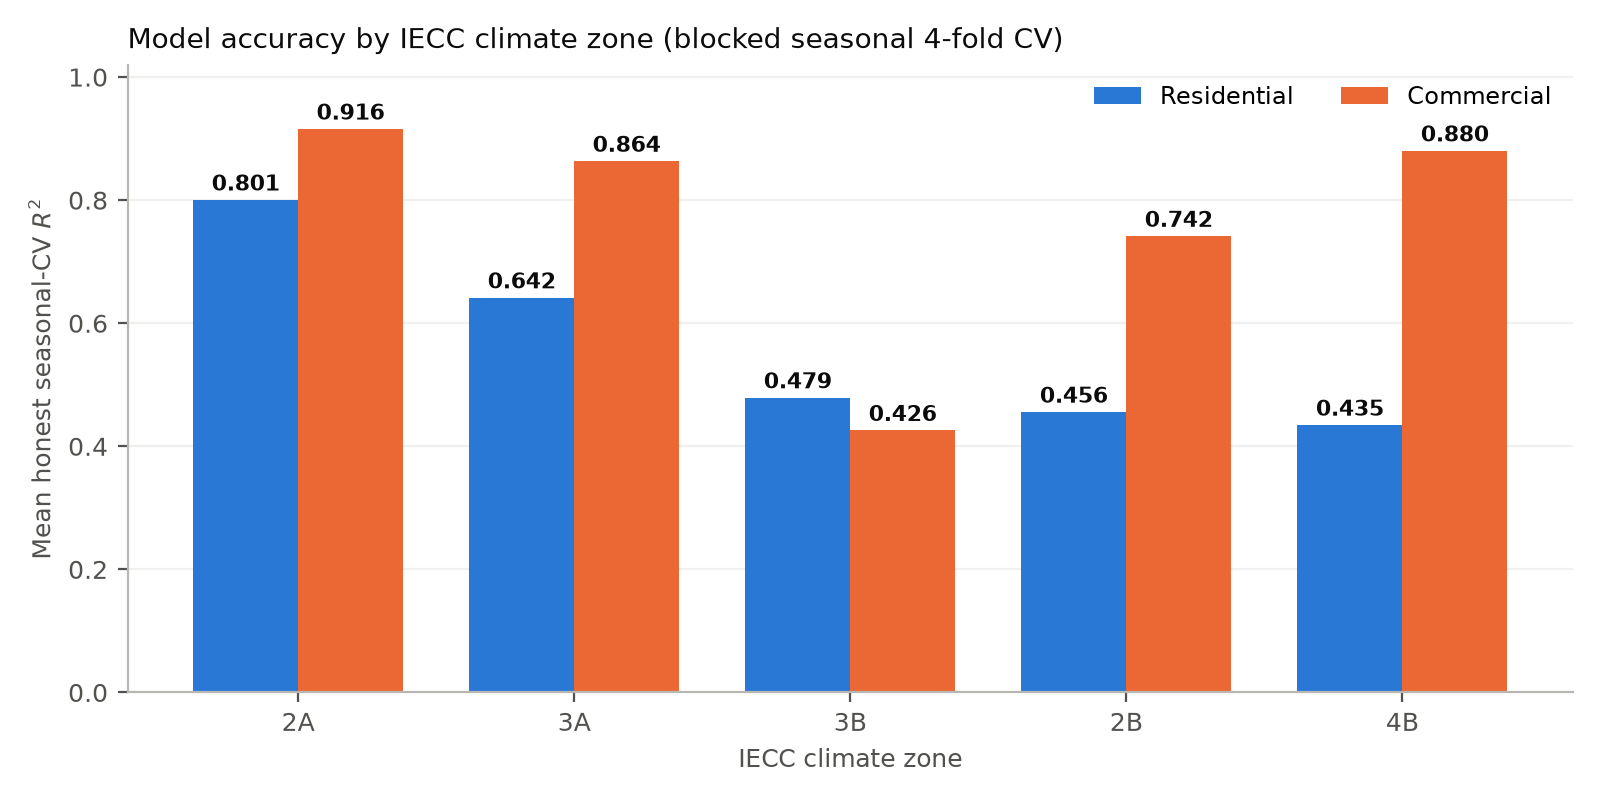
\includegraphics[width=0.82\textwidth]{figures/statewide_r2_by_zone_fig1.png}
\caption{Model accuracy by climate zone. Commercial exceeds residential everywhere except
zone 3B, where hotel and grocery archetypes carry genuinely no weather signal (Permian oilfield
workforce cycles); four 3B/2B archetype combinations have negative mean $R^2$.}
\label{fig:r2}
\end{figure}

\section{Spatial allocation: effect of the area split}

\begin{table}[H]
\centering\small
\begin{tabular}{lcc}
\toprule
& Nearest-bus join & Area-split \\
\midrule
\multicolumn{3}{l}{\emph{Residential, 50 parts per tract}}\\
\quad Tracts split across $>$1 bus & 0\% & 84.0\% \\
\quad Buses receiving dwellings & 3{,}426 & \textbf{6{,}352} \\
\quad Load-carrying buses with zero dwellings & 1{,}824 & \textbf{25} \\
\quad Spearman $\rho$ vs.\ bus \texttt{Load\_MW} & 0.502 & \textbf{0.606} \\
\midrule
\multicolumn{3}{l}{\emph{Commercial, 100 parts per ZCTA}}\\
\quad ZCTAs split across $>$1 bus & 0\% & 90.2\% \\
\quad Buses receiving floor space & 1{,}598 & \textbf{6{,}329} \\
\quad Load-carrying buses with commercial load & 20.1\% & \textbf{96.1\%} \\
\quad Spearman $\rho$ vs.\ bus \texttt{Load\_MW} & 0.133 & \textbf{0.475} \\
\bottomrule
\end{tabular}
\caption{Scored against the Texas 7k case's own per-bus \texttt{Load\_MW}. Spearman rather than
Pearson: \texttt{Load\_MW} also contains industrial demand, so a few very large industrial buses
dominate any linear correlation.}
\label{tab:areasplit}
\end{table}

\begin{figure}[H]
\centering
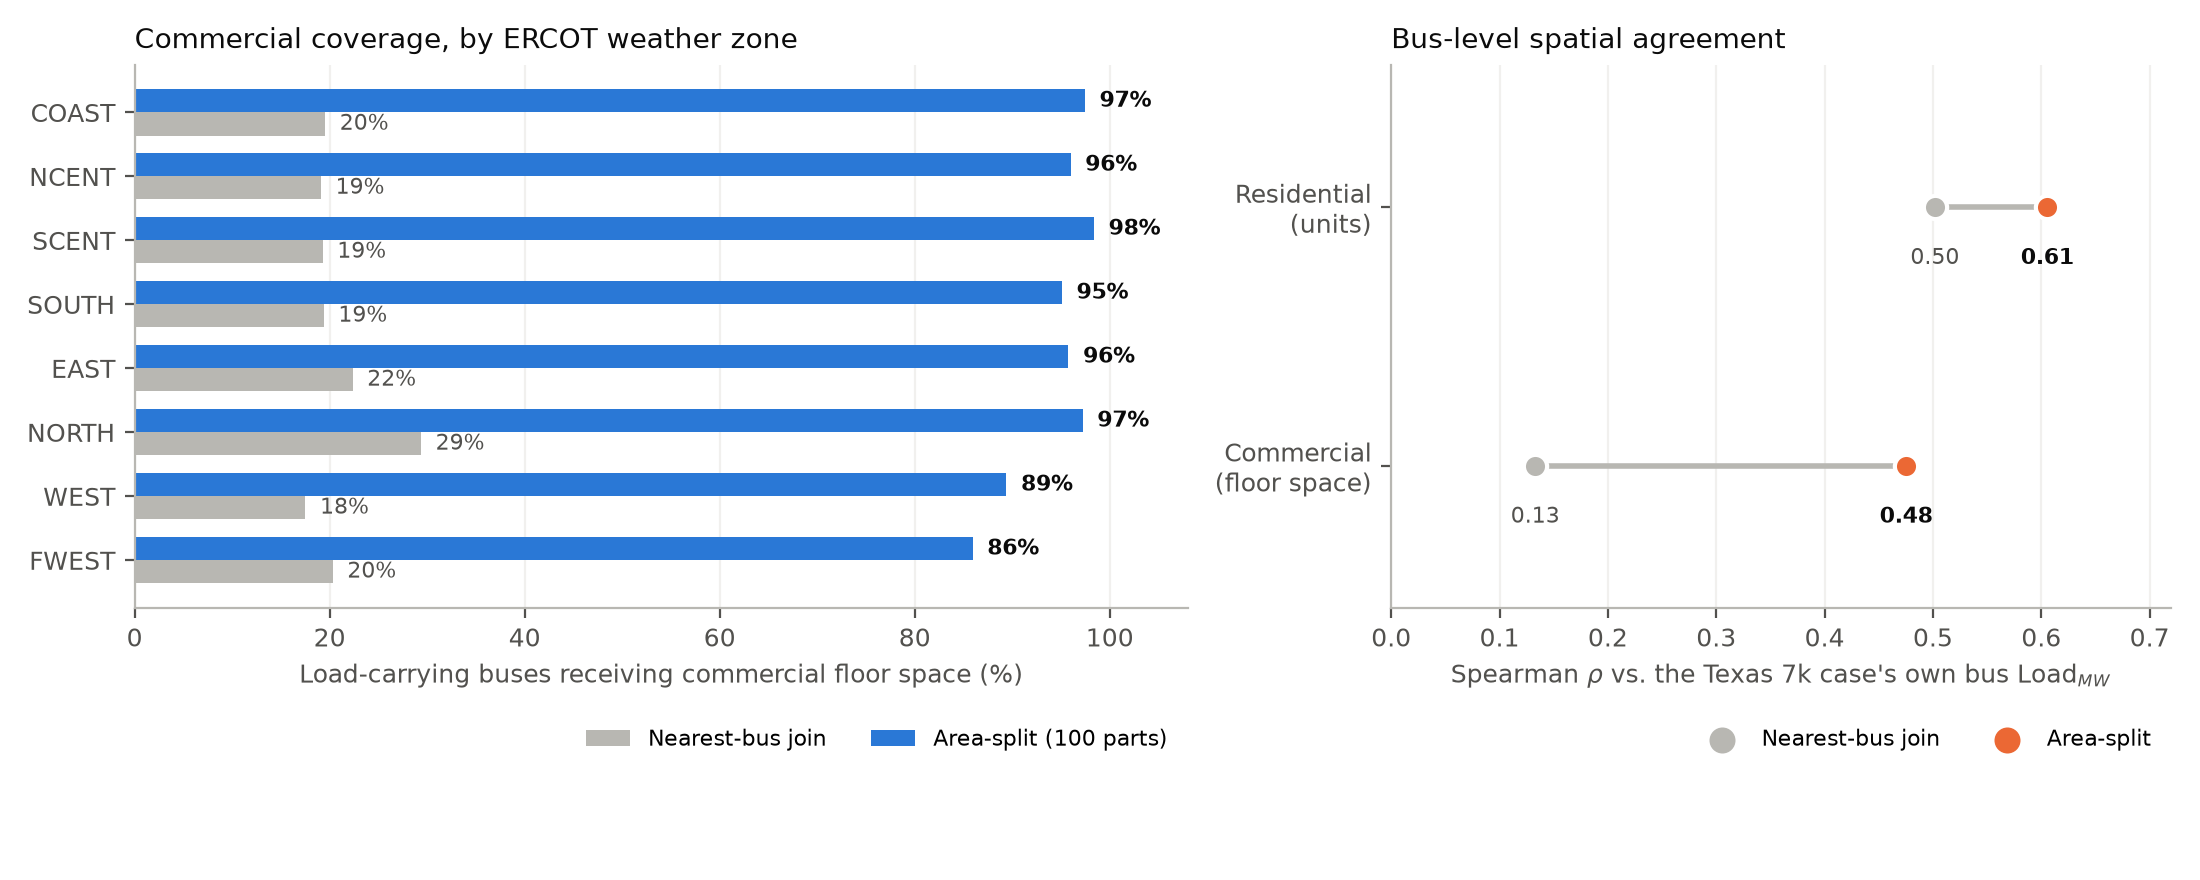
\includegraphics[width=\textwidth]{figures/area_split_fig1.png}
\caption{Left: share of load-carrying buses receiving commercial floor space, by ERCOT zone.
Right: bus-level rank agreement with the case's own per-bus load.}
\label{fig:areasplit}
\end{figure}

\paragraph{Worth stating in the paper.} This improvement is \emph{invisible} to every
zone-aggregate metric: redistributing load among buses of the same zone leaves that zone's total
unchanged (zone totals moved by $-1.6\%$ to $+7.8\%$, most under 2\%). Bus-level fidelity is what
the framework exists to produce, so a validation protocol based only on aggregate correlation
would miss it entirely --- which is the argument for reporting the \texttt{Load\_MW} rank
statistic alongside the usual metrics.

\section{Validation against ERCOT}

\subsection{Per-zone and statewide}

\begin{table}[H]
\centering\small
\begin{tabular}{lrrrrrr}
\toprule
ERCOT zone & ERCOT peak & Recon.\ peak & Peak ratio & LF (ERCOT) & LF (recon.) & Pearson $r$ \\
 & (MW) & (MW) & & & & \\
\midrule
COAST & 20{,}269.8 & 19{,}613.6 & 0.97 & 0.600 & 0.620 & 0.900 \\
NCENT & 26{,}499.2 & 27{,}100.4 & 1.02 & 0.524 & 0.512 & 0.901 \\
SCENT & 14{,}166.7 & 12{,}650.0 & 0.89 & 0.484 & 0.542 & 0.902 \\
SOUTH & 6{,}176.1 & 5{,}734.7 & 0.93 & 0.577 & 0.621 & 0.911 \\
WEST & 2{,}083.6 & 1{,}919.7 & 0.92 & 0.612 & 0.664 & 0.823 \\
FWEST & 3{,}655.0 & 3{,}471.3 & 0.95 & 0.782 & 0.824 & \textbf{0.655} \\
EAST$^\dagger$ & 2{,}620.8 & 2{,}700.1 & --- & 0.569 & 0.552 & 0.911 \\
NORTH$^\dagger$ & 1{,}521.8 & 1{,}415.5 & --- & 0.571 & 0.614 & 0.905 \\
\midrule
\textbf{STATEWIDE} & \textbf{73{,}308.2} & \textbf{72{,}617.0} & \textbf{0.99} & \textbf{0.586} & \textbf{0.592} & \textbf{0.922} \\
\bottomrule
\end{tabular}
\caption{Calibrated reconstruction vs.\ ERCOT actual load, 2018. $^\dagger$The synthetic case's
EAST and NORTH area boundaries do not coincide with ERCOT's (their case peak load is
1.33$\times$ and 2.21$\times$ the ERCOT zonal peak), so their shape statistics are interpretable
but their magnitudes are not.}
\label{tab:validation}
\end{table}

\begin{figure}[H]
\centering
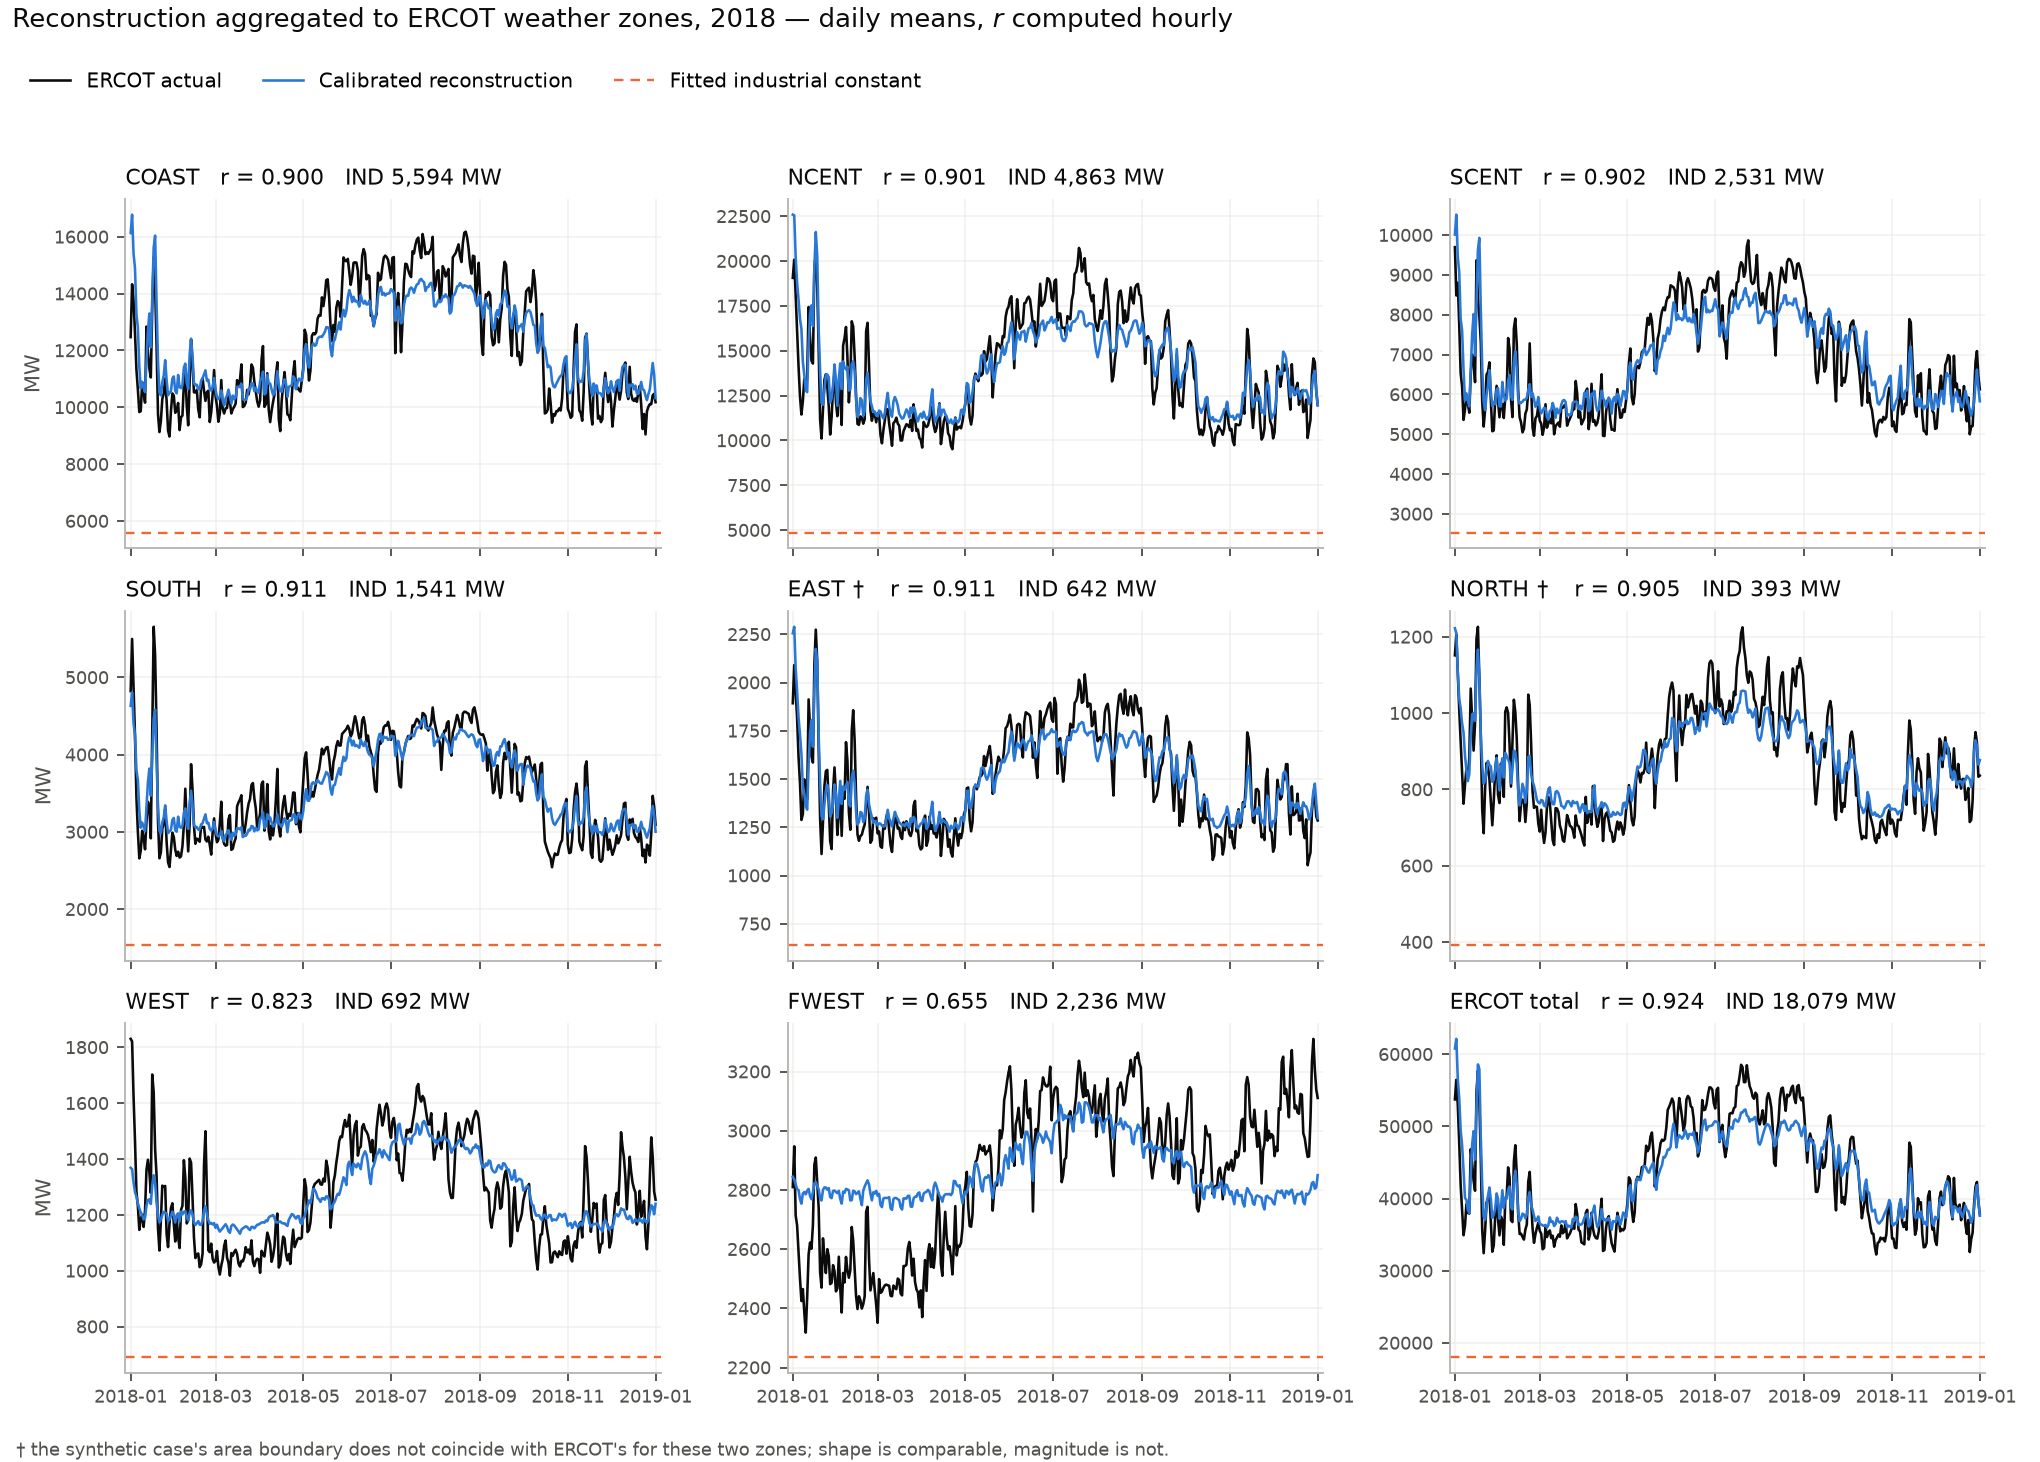
\includegraphics[width=\textwidth]{figures/ercot_8zone_fig1.png}
\caption{Calibrated reconstruction aggregated to each ERCOT weather zone. Daily means plotted
for legibility; $r$ computed hourly.}
\label{fig:8zone}
\end{figure}

\subsection{Calibration coefficients}

\begin{table}[H]
\centering\small
\begin{tabular}{lrrrr}
\toprule
ERCOT zone & RES & COM & IND (MW) & IND as \% of zone peak \\
\midrule
COAST & 1.07 & 0.98 & 5{,}594 & 27.6 \\
NCENT & 1.36 & 0.98 & 4{,}863 & 18.4 \\
SCENT & 1.26 & 0.00$^{\ast}$ & 2{,}531 & 17.9 \\
SOUTH & 1.14 & 0.66 & 1{,}541 & 25.0 \\
WEST & 1.07 & 3.03$^{\ast}$ & 692 & 33.2 \\
FWEST & \textbf{0.30} & 1.46 & 2{,}236 & \textbf{61.2} \\
EAST$^\dagger$ & 0.58 & 0.70 & 642 & 24.5 \\
NORTH$^\dagger$ & 0.58 & 0.77 & 393 & 25.8 \\
\midrule
\textbf{Statewide fit} & \textbf{1.15} & \textbf{0.76} & \textbf{18{,}079} & \textbf{24.7} \\
\bottomrule
\end{tabular}
\caption{Per-zone calibration, NNLS, scored by blocked seasonal CV. $^{\ast}$see
Section~\ref{sec:limits}.}
\label{tab:calibration}
\end{table}

\begin{figure}[H]
\centering
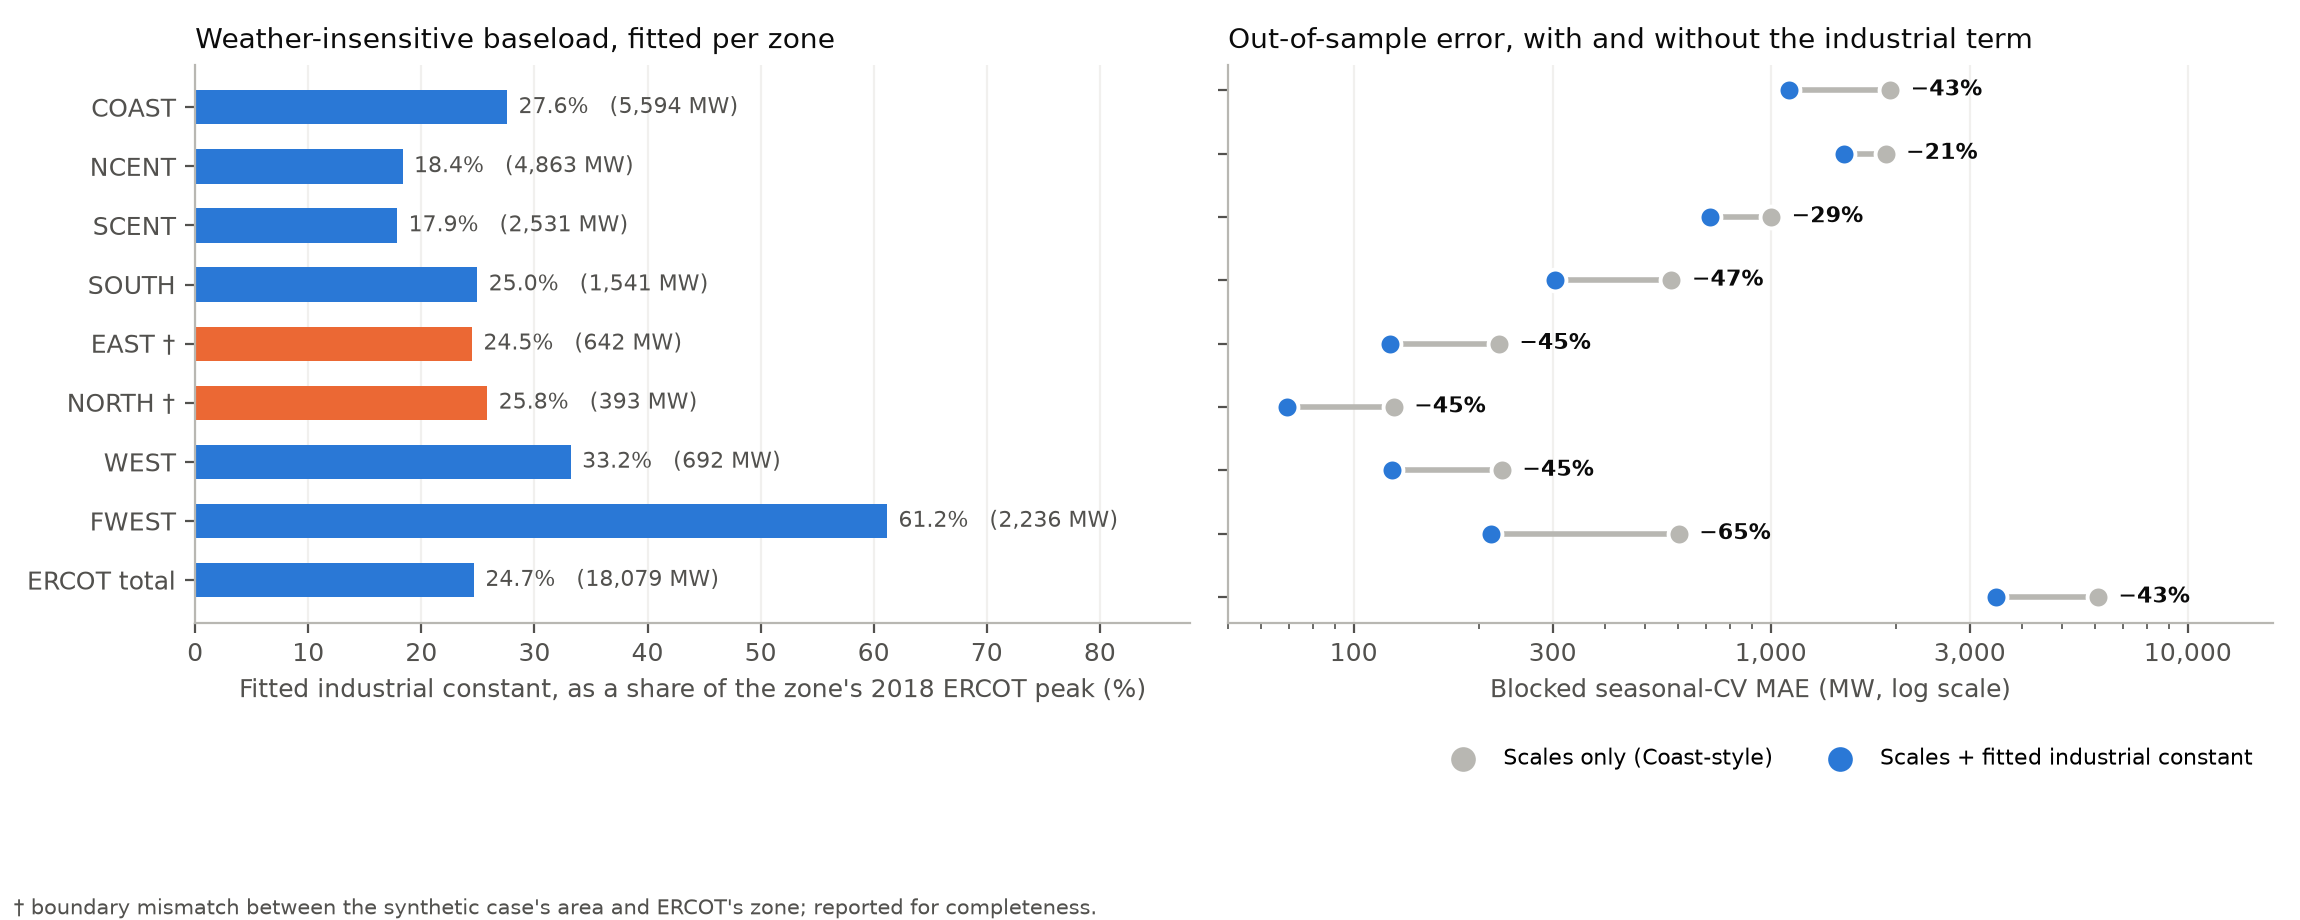
\includegraphics[width=\textwidth]{figures/zone_calibration_fig1.png}
\caption{Left: fitted weather-insensitive baseload as a share of each zone's ERCOT peak.
Right: out-of-sample error with and without the industrial term.}
\label{fig:calibration}
\end{figure}

\paragraph{Three results to carry into the paper.}
\begin{enumerate}
\item \textbf{The building-stock reconstruction needs almost no fudge factor.} With an industrial
term present, $\mathrm{RES}$ sits at 1.07--1.36 in five of the six well-matched zones, against
1.6--1.9 for Coast without one. The earlier large scale factors were compensating for a missing
\emph{load component}, not for a mis-sized housing stock.
\item \textbf{Industrial demand is roughly a quarter of ERCOT} (18{,}079\,MW statewide, 24.7\% of
system peak). Coast alone fits 5{,}594\,MW, which retrospectively validates the hand-picked
4{,}500\,MW placeholder as the right order of magnitude and slightly low.
\item \textbf{FWEST is structurally industrial}: $\mathrm{RES}=0.30$ and an industrial constant
equal to 61.2\% of its peak --- a quantitative explanation for its weak correlation, and the
clearest evidence that a weather-driven reconstruction cannot track Permian load.
\end{enumerate}

\section{Validation metrics beyond aggregate correlation}

The metric suite requested in review point 5, computed statewide with the same definitions used
for Coast.

\begin{figure}[H]
\centering
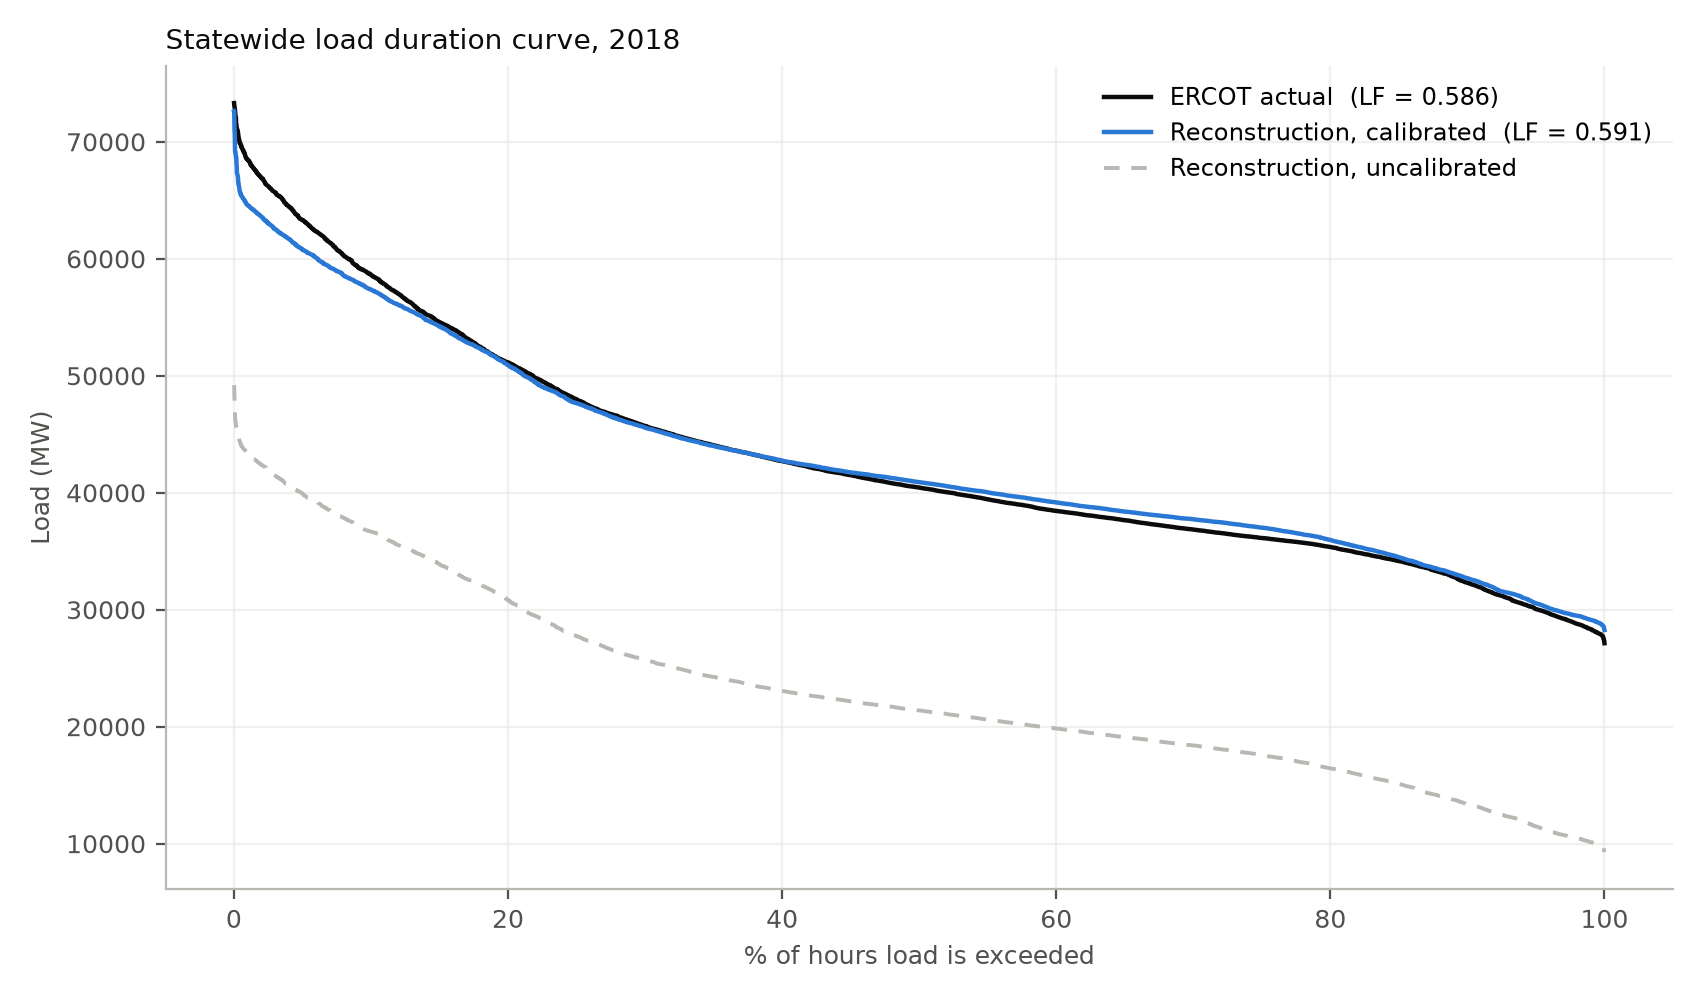
\includegraphics[width=0.85\textwidth]{figures/statewide_ldc_fig1.png}
\caption{Load duration curve. The calibrated curve tracks ERCOT across the whole range; the load
factor matches to within 0.006 (0.592 vs.\ 0.586), against 0.556 vs.\ 0.600 for the Coast study.}
\label{fig:ldc}
\end{figure}

\begin{figure}[H]
\centering
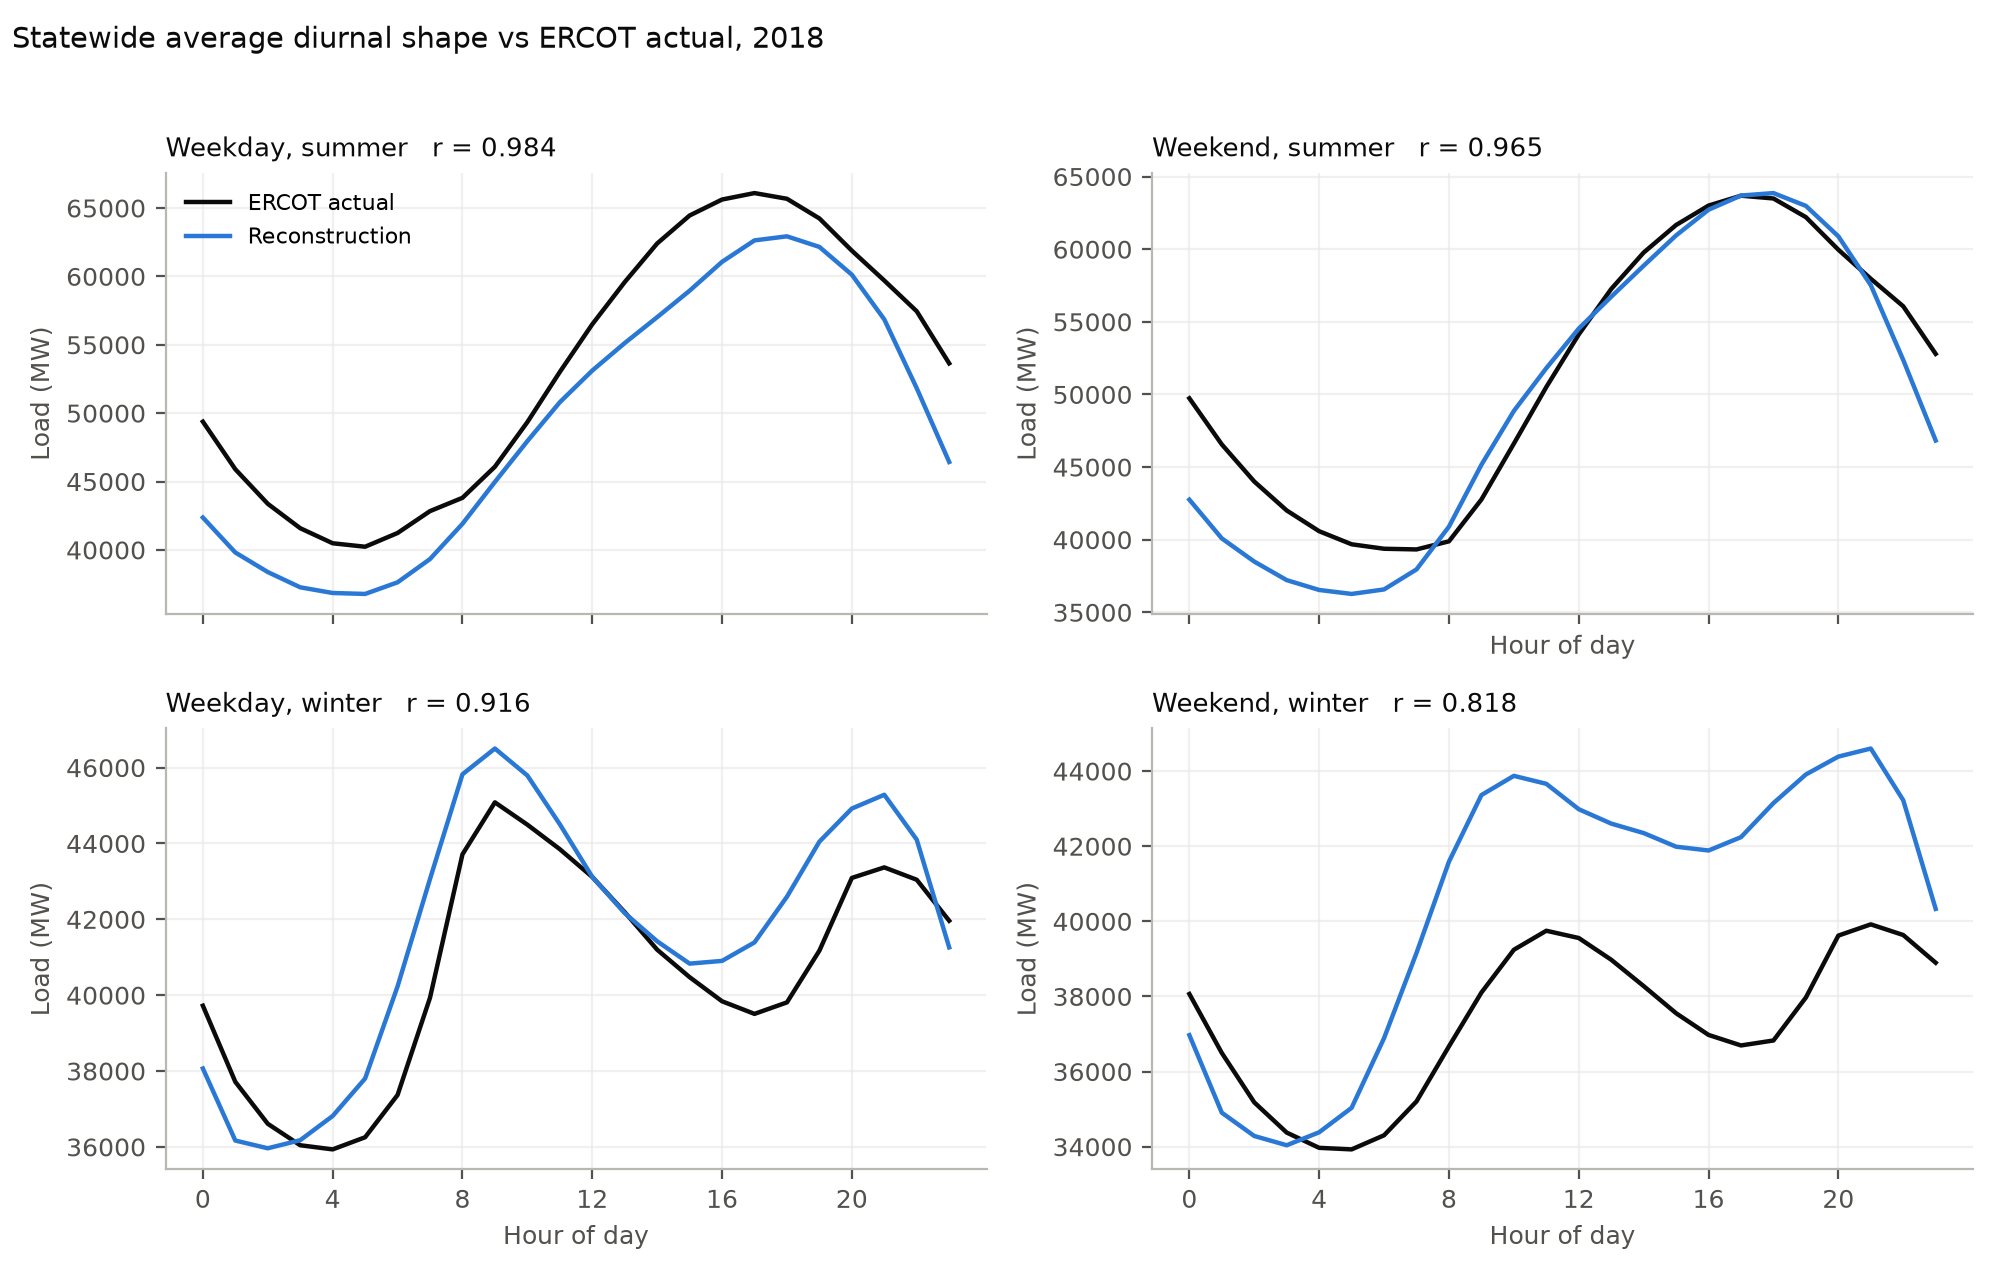
\includegraphics[width=\textwidth]{figures/statewide_diurnal_fig1.png}
\caption{Average diurnal shape. Summer is reproduced almost exactly ($r=0.984$ weekday,
$0.965$ weekend); winter weekend remains the weakest condition ($r=0.818$), as it was for Coast.}
\label{fig:diurnal}
\end{figure}

\begin{figure}[H]
\centering
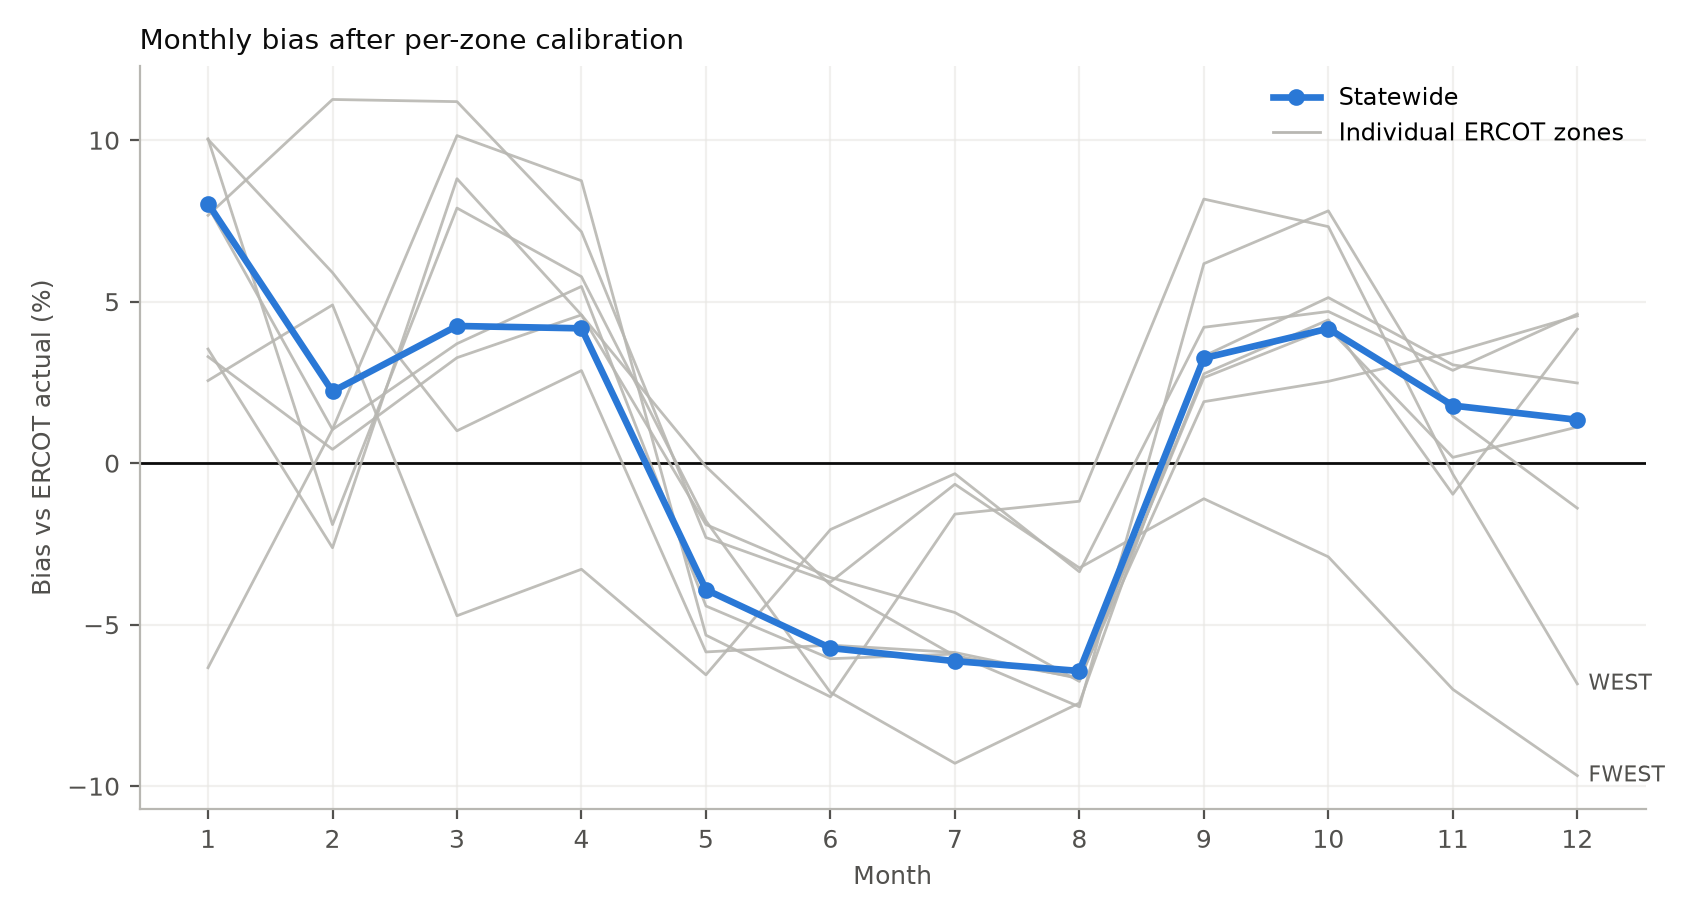
\includegraphics[width=0.85\textwidth]{figures/statewide_monthly_bias_fig1.png}
\caption{Monthly bias. Statewide bias stays within $-6.4\%$ (August) and $+8.0\%$ (January),
mean absolute 4.3\%, and changes sign across the year --- a shape residual, not a scale error.
The Coast study's bias was positive in every month and ranged $+10.5\%$ to $+29.8\%$.}
\label{fig:bias}
\end{figure}

\begin{table}[H]
\centering\small
\begin{tabular}{lccc}
\toprule
Scope & CF residential & CF commercial & CF combined \\
\midrule
\textbf{Statewide (6{,}717 buses)} & \textbf{0.954} & \textbf{0.975} & \textbf{0.941} \\
\midrule
COAST & 1.000 & 0.997 & 0.990 \\
NCENT & 0.992 & 0.998 & 0.992 \\
SCENT & 0.981 & n/a$^{\ast}$ & 0.981 \\
SOUTH & 0.854 & 0.970 & 0.875 \\
WEST & 0.899 & 0.975 & 0.926 \\
FWEST & 0.993 & 0.998 & 0.978 \\
EAST$^\dagger$ & 0.987 & 0.994 & 0.983 \\
NORTH$^\dagger$ & 0.897 & 0.985 & 0.886 \\
\bottomrule
\end{tabular}
\caption{Coincidence factor (system peak / sum of individual bus peaks); diversity factor is its
reciprocal, so the statewide combined DF is 1.063. $^{\ast}$undefined: SCENT's fitted
$\mathrm{COM}=0$ makes the commercial stack identically zero.}
\label{tab:cf}
\end{table}

\paragraph{The coincidence factor is finally informative.} In the Coast study it sat at
0.96--1.00 across every pipeline version --- a structural artifact of all 200 buses sharing one
zone-wide weather series, not a physical result. Statewide, buses span eight weather zones and
five climate zones, and the combined CF drops to \textbf{0.941}. Within a single zone it is still
near 1 (COAST 0.990, NCENT 0.992), so the diversity being measured is \emph{between} climate
zones, not between buses. That is an honest reading, and it identifies per-bus weather
granularity as the remaining lever.

\begin{table}[H]
\centering\small
\begin{tabular}{lcc}
\toprule
Spatial consistency proxy & Coast (200 buses) & Statewide (6{,}717 buses) \\
\midrule
Residential annual energy vs.\ dwellings & 0.948 & \textbf{0.973} \\
Commercial annual energy vs.\ floor space & 0.892 & \textbf{0.971} \\
\bottomrule
\end{tabular}
\caption{Correlation between per-bus annual energy and its per-bus driver. The commercial jump
is the area split: under the nearest-ZCTA join most buses had zero floor space but non-zero
modelled energy.}
\label{tab:spatial}
\end{table}

\section{Limitations to state explicitly}
\label{sec:limits}

\begin{enumerate}
\item \textbf{Industrial load is a constant, not a model.} It is fitted rather than assumed, which
is an improvement, but it cannot reproduce industrial load's own temporal variation. This caps
FWEST at $r=0.655$ and WEST at $0.823$. A time-varying, data-driven industrial representation is
the single most consequential remaining gap.
\item \textbf{The area split assumes uniform density within a polygon.} Equal-area subdivision is
a weak assumption in large rural tracts with one town, and nearly harmless in dense urban ones ---
which is where most load sits. It is still strictly better than assigning a whole polygon to one
bus, and \texttt{Load\_MW} now provides a per-bus reference to quantify the residual.
\item \textbf{EAST and NORTH have boundary mismatches.} The synthetic case's area load is
1.33$\times$ and 2.21$\times$ their ERCOT peak, so only their shapes are comparable.
\item \textbf{South Central fits $\mathrm{COM}=0$ and West fits 3.03.} For SCENT, the partial
correlation of the commercial profile with ERCOT load (residential removed) is $-0.014$, against
$+0.24$ to $+0.34$ in every other zone: the commercial stack genuinely adds no information there.
Poor coverage and collinearity were both tested and ruled out (coverage is now 96\%; VIF
$\approx1.9$). Unexplained, and isolated to the Austin/San~Antonio corridor.
\item \textbf{All buses in a zone share one weather series.} Table~\ref{tab:cf} shows the
consequence directly: within-zone coincidence factors remain near 1. Per-bus or per-county
weather is the natural next refinement.
\item \textbf{Four archetype/zone combinations have negative $R^2$} (3B largehotel $-1.36$,
3B smallhotel $-0.28$, 2B smallhotel $-0.26$, 3B grocery $-0.10$). These are lumpy, low-signal
archetypes in oilfield regions; worth excluding from calibration rather than letting them
contribute noise.
\end{enumerate}

\section*{Where the numbers live}

Every figure here is in \texttt{latex\_report/figures/}; every table is backed by a CSV in
\texttt{statewide/metrics/}:
\texttt{statewide\_validation\_summary.csv} (Table~\ref{tab:validation}),
\texttt{zone\_calibration.csv} (Table~\ref{tab:calibration}),
\texttt{statewide\_coincidence\_diversity.csv} (Table~\ref{tab:cf}),
\texttt{statewide\_monthly\_bias.csv}, \texttt{statewide\_diurnal\_corr.csv},
\texttt{statewide\_spatial\_proxy.csv}, and \texttt{seasonal\_cv\_\{ZONE\}.csv} plus
\texttt{seasonal\_cv\_comstock\_\{ZONE\}.csv} (Table~\ref{tab:r2}). Reproduce with
\texttt{statewide/notebooks/}: \texttt{00\_zone\_mapping} $\rightarrow$
\texttt{residential\_\{ZONE\}} and \texttt{commercial\_\{ZONE\}} $\rightarrow$
\texttt{zone\_calibration} $\rightarrow$ \texttt{validation\_metrics\_statewide}.

\end{document}
